\documentclass{ximera}

 

\usepackage{epsfig}

\graphicspath{
  {./}
  {figures/}
}

\usepackage{morewrites}
\makeatletter
\newcommand\subfile[1]{%
\renewcommand{\input}[1]{}%
\begingroup\skip@preamble\otherinput{#1}\endgroup\par\vspace{\topsep}
\let\input\otherinput}
\makeatother

\newcommand{\includeexercises}{\directlua{dofile("/home/jim/linearAlgebra/laode/exercises.lua")}}

%\newcounter{ccounter}
%\setcounter{ccounter}{1}
%\newcommand{\Chapter}[1]{\setcounter{chapter}{\arabic{ccounter}}\chapter{#1}\addtocounter{ccounter}{1}}

%\newcommand{\section}[1]{\section{#1}\setcounter{thm}{0}\setcounter{equation}{0}}

%\renewcommand{\theequation}{\arabic{chapter}.\arabic{section}.\arabic{equation}}
%\renewcommand{\thefigure}{\arabic{chapter}.\arabic{figure}}
%\renewcommand{\thetable}{\arabic{chapter}.\arabic{table}}

%\newcommand{\Sec}[2]{\section{#1}\markright{\arabic{ccounter}.\arabic{section}.#2}\setcounter{equation}{0}\setcounter{thm}{0}\setcounter{figure}{0}}

\newcommand{\Sec}[2]{\section{#1}}

\setcounter{secnumdepth}{2}
%\setcounter{secnumdepth}{1} 

%\newcounter{THM}
%\renewcommand{\theTHM}{\arabic{chapter}.\arabic{section}}

\newcommand{\trademark}{{R\!\!\!\!\!\bigcirc}}
%\newtheorem{exercise}{}

\newcommand{\dfield}{{\sf dfield9}}
\newcommand{\pplane}{{\sf pplane9}}

\newcommand{\EXER}{\section*{Exercises}}%\vspace*{0.2in}\hrule\small\setcounter{exercise}{0}}
\newcommand{\CEXER}{}%\vspace{0.08in}\begin{center}Computer Exercises\end{center}}
\newcommand{\TEXER}{} %\vspace{0.08in}\begin{center}Hand Exercises\end{center}}
\newcommand{\AEXER}{} %\vspace{0.08in}\begin{center}Hand Exercises\end{center}}

% BADBAD: \newcommand{\Bbb}{\bf}

\newcommand{\R}{\mbox{$\Bbb{R}$}}
\newcommand{\C}{\mbox{$\Bbb{C}$}}
\newcommand{\Z}{\mbox{$\Bbb{Z}$}}
\newcommand{\N}{\mbox{$\Bbb{N}$}}
\newcommand{\D}{\mbox{{\bf D}}}
\usepackage{amssymb}
%\newcommand{\qed}{\hfill\mbox{\raggedright$\square$} \vspace{1ex}}
%\newcommand{\proof}{\noindent {\bf Proof:} \hspace{0.1in}}

\newcommand{\setmin}{\;\mbox{--}\;}
\newcommand{\Matlab}{{M\small{AT\-LAB}} }
\newcommand{\Matlabp}{{M\small{AT\-LAB}}}
\newcommand{\computer}{\Matlab Instructions}
\newcommand{\half}{\mbox{$\frac{1}{2}$}}
\newcommand{\compose}{\raisebox{.15ex}{\mbox{{\scriptsize$\circ$}}}}
\newcommand{\AND}{\quad\mbox{and}\quad}
\newcommand{\vect}[2]{\left(\begin{array}{c} #1_1 \\ \vdots \\
 #1_{#2}\end{array}\right)}
\newcommand{\mattwo}[4]{\left(\begin{array}{rr} #1 & #2\\ #3
&#4\end{array}\right)}
\newcommand{\mattwoc}[4]{\left(\begin{array}{cc} #1 & #2\\ #3
&#4\end{array}\right)}
\newcommand{\vectwo}[2]{\left(\begin{array}{r} #1 \\ #2\end{array}\right)}
\newcommand{\vectwoc}[2]{\left(\begin{array}{c} #1 \\ #2\end{array}\right)}

\newcommand{\ignore}[1]{}


\newcommand{\inv}{^{-1}}
\newcommand{\CC}{{\cal C}}
\newcommand{\CCone}{\CC^1}
\newcommand{\Span}{{\rm span}}
\newcommand{\rank}{{\rm rank}}
\newcommand{\trace}{{\rm tr}}
\newcommand{\RE}{{\rm Re}}
\newcommand{\IM}{{\rm Im}}
\newcommand{\nulls}{{\rm null\;space}}

\newcommand{\dps}{\displaystyle}
\newcommand{\arraystart}{\renewcommand{\arraystretch}{1.8}}
\newcommand{\arrayfinish}{\renewcommand{\arraystretch}{1.2}}
\newcommand{\Start}[1]{\vspace{0.08in}\noindent {\bf Section~\ref{#1}}}
\newcommand{\exer}[1]{\noindent {\bf \ref{#1}}}
\newcommand{\ans}{}
\newcommand{\matthree}[9]{\left(\begin{array}{rrr} #1 & #2 & #3 \\ #4 & #5 & #6
\\ #7 & #8 & #9\end{array}\right)}
\newcommand{\cvectwo}[2]{\left(\begin{array}{c} #1 \\ #2\end{array}\right)}
\newcommand{\cmatthree}[9]{\left(\begin{array}{ccc} #1 & #2 & #3 \\ #4 & #5 &
#6 \\ #7 & #8 & #9\end{array}\right)}
\newcommand{\vecthree}[3]{\left(\begin{array}{r} #1 \\ #2 \\
#3\end{array}\right)}
\newcommand{\cvecthree}[3]{\left(\begin{array}{c} #1 \\ #2 \\
#3\end{array}\right)}
\newcommand{\cmattwo}[4]{\left(\begin{array}{cc} #1 & #2\\ #3
&#4\end{array}\right)}

\newcommand{\Matrix}[1]{\ensuremath{\left(\begin{array}{rrrrrrrrrrrrrrrrrr} #1 \end{array}\right)}}

\newcommand{\Matrixc}[1]{\ensuremath{\left(\begin{array}{cccccccccccc} #1 \end{array}\right)}}



\renewcommand{\labelenumi}{\theenumi)}
\newenvironment{enumeratea}%
{\begingroup
 \renewcommand{\theenumi}{\alph{enumi}}
 \renewcommand{\labelenumi}{(\theenumi)}
 \begin{enumerate}}
 {\end{enumerate}\endgroup}



\newcounter{help}
\renewcommand{\thehelp}{\thesection.\arabic{equation}}

%\newenvironment{equation*}%
%{\renewcommand\endequation{\eqno (\theequation)* $$}%
%   \begin{equation}}%
%   {\end{equation}\renewcommand\endequation{\eqno \@eqnnum
%$$\global\@ignoretrue}}

%\input{psfig.tex}

\author{Martin Golubitsky and Michael Dellnitz}

%\newenvironment{matlabEquation}%
%{\renewcommand\endequation{\eqno (\theequation*) $$}%
%   \begin{equation}}%
%   {\end{equation}\renewcommand\endequation{\eqno \@eqnnum
% $$\global\@ignoretrue}}

\newcommand{\soln}{\textbf{Solution:} }
\newcommand{\exercap}[1]{\centerline{Figure~\ref{#1}}}
\newcommand{\exercaptwo}[1]{\centerline{Figure~\ref{#1}a\hspace{2.1in}
Figure~\ref{#1}b}}
\newcommand{\exercapthree}[1]{\centerline{Figure~\ref{#1}a\hspace{1.2in}
Figure~\ref{#1}b\hspace{1.2in}Figure~\ref{#1}c}}
\newcommand{\para}{\hspace{0.4in}}

\renewenvironment{solution}{\suppress}{\endsuppress}

\ifxake
\newenvironment{matlabEquation}{\begin{equation}}{\end{equation}}
\else
\newenvironment{matlabEquation}%
{\let\oldtheequation\theequation\renewcommand{\theequation}{\oldtheequation*}\begin{equation}}%
  {\end{equation}\let\theequation\oldtheequation}
\fi

\makeatother


\title{Higher Dimensional Systems Using ode45}

\begin{document}
\begin{abstract}
\end{abstract}
\maketitle

\label{S:ode45HD}

In this section we discuss how to use {\tt ode45} to find solutions to linear
and nonlinear systems of differential equations in three dimensions, and how 
to plot the results of these calculations.  The same ideas will work in 
principle in any numbers of dimensions.  Specifically, we compute the solutions 
of a nonlinear system and its linearization at a hyperbolic equilibrium.  In 
this example we test numerically the conclusions of 
Theorem~\ref{T:nlinearization} on linearized stability for nonlinear systems.

 
\subsubsection*{A Three Dimensional Linear Example}

We now use {\tt ode45} to numerically compute solutions of the system
$\dot{X} = AX$ where 
\begin{equation}  \label{E:3dexample}
A = \left(\begin{array}{rrr}
  -0.25 & 3.00 & 0\\
   -3.00 & -0.25 &  0\\
   0 &  0 & -0.2
\end{array}\right).
\end{equation}
The function  
\begin{matlabEquation}\label{MATLAB:54}
f(X) = AX
\end{matlabEquation}
that is on the right hand side of this linear system of differential 
equations is stored in the m-file {\tt f14\_4\_2.m}.  The following lines 
are included in that m-file.
\begin{verbatim}
function f = f14_4_2(t,x)
A = [ -0.25 3.0 0; -3 -0.25 0; 0 0 -0.2];
f = A*x;
\end{verbatim}
Observe that the first argument of the function {\tt f14\_4\_2} has to be 
$t$ even though this variable does not explicitly occur on the right hand 
side.  

The eigenvalues of $A$ are $-0.25\pm 3i$ and $-0.2$.  It follows that in the 
$x_1x_2$ plane solutions spiral into the origin and along the $x_3$ axis 
solutions decay exponentially to the origin.  By superpositon most solutions
will spiral around the $x_3$ axis while decaying into the origin.  We test 
this prediction using {\tt ode45}.

We approximate the solution starting in $X_0=(2,-1,-1)$ using
{\tt ode45} on the time interval $[0,100]$ by typing
\begin{verbatim}
[t,x] = ode45('f14_4_2',[0 100],[2,-1,-1]');
\end{verbatim}
Note that when using {\tt ode45},\index{\computer!ode45} the 
initial condition must be entered 
as a {\em column\/} vector.   (The reason is that this vector is an
input argument of the function {\tt f14\_4\_2} and in this function
this argument is multiplied by the matrix {\tt A}.)  When the computation 
is complete, 
the approximation of $(t,x_1(t),x_2(t),x_3(t))$ is stored in the column 
vector {\tt t} and in the three columns of the matrix {\tt x}.  Indeed, if 
we type {\tt size(t)} or {\tt size(x)}, then we see that {\tt t} is a 
vector of length $897$ and {\tt x} is a matrix with $897$ rows and $3$ 
columns.  

Next we consider how to graphically view the solutions.  As in one and
two dimensions, there are two possibilities.  First, we can visualize 
the three time series\index{time series} 
$(t,x_1(t))$, $(t,x_2(t))$ and $(t,x_3(t))$.  
This can be done by typing
\begin{verbatim}
subplot(3,1,1)
plot(t,x(:,1))
ylabel('x1')
subplot(3,1,2)
plot(t,x(:,2))
ylabel('x2')
subplot(3,1,3)
plot(t,x(:,3))
ylabel('x3')
xlabel('t')
\end{verbatim}
\index{\computer!subplot}\index{\computer!plot}
We then obtain the result shown in Figure~\ref{fig:flinear1}.  This figure 
shows the expected oscillation in the $x_1$ and $x_2$ coordinates and the 
exponential decay in the $x_3$ coordinate.
\begin{figure*}[htb]
   \centerline{%
   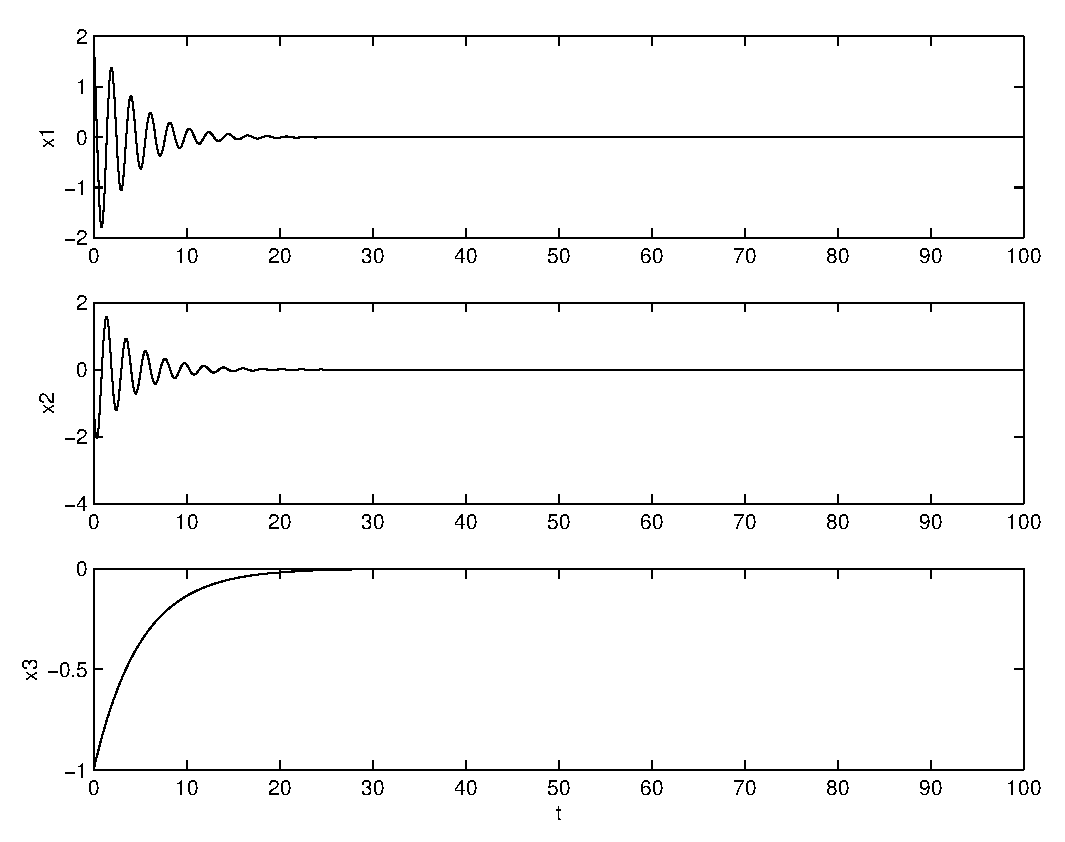
\psfig{file=../figures/flinear1.eps,width=5.6in,height=2.8in}}
   \caption{Time series showing convergence to the origin for the solution 
	of the linear system $\dot X=AX$, where $A$ is as in 
	\protect\eqref{E:3dexample}, with initial condition $X_0=(2,-1,-1)$.}
   \label{fig:flinear1}
\end{figure*}

In drawing Figure~\ref{fig:flinear1} we have introduced another \Matlab 
graphics command {\tt subplot(m,n,p)}\index{\computer!subplot}.  
The {\tt subplot} command activates one 
subfigure in an $m\times n$ matrix of subfigures.  In this case $m=3$ 
and $n=1$ so that we produce three subfigures arranged vertically.  
The number $p$ indicates which subfigure is the active subfigure --- the 
subfigure to which the {\tt plot} command refers.

The second possibility for the graphical representation of the solution
is the phase space plot.  Here we visualize the curve
$(x_1(t),x_2(t),x_3(t))$ in three dimensional space by typing
\begin{verbatim}
clf
plot3(x(:,1),x(:,2),x(:,3))
xlabel('x1')
ylabel('x2')
zlabel('x3')
\end{verbatim}\index{\computer!clf}\index{\computer!plot3}\index{\computer!xlabel}
\index{\computer!ylabel}\index{\computer!zlabel}
The result is shown in Figure~\ref{fig:flinear2}.  Note that we begin by 
using the \Matlab graphics command {\tt clf} to clear all previous graphics.
\begin{figure}[htb]
   \centerline{%
   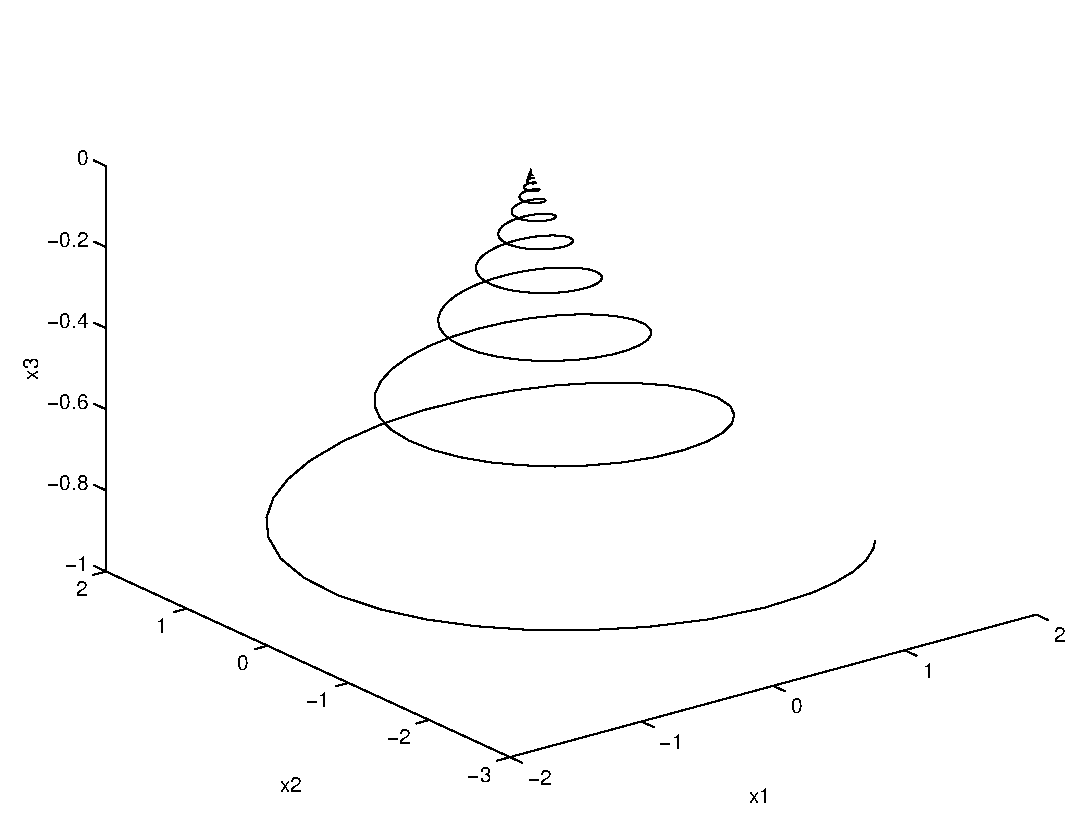
\psfig{file=../figures/flinear2.eps,width=3.6in}}
   \caption{Phase space plot showing convergence to the origin for the 
	solution of the linear system $\dot X=AX$, where $A$ is as in 
	\protect\eqref{E:3dexample}, with initial condition $X_0=(2,-1,-1)$.}
   \label{fig:flinear2}
\end{figure}


\subsubsection*{A Three Dimensional Nonlinear System}

We now solve the nonlinear differential equation 
\begin{matlabEquation}  \label{E:fnonlin}
\dot{X} = AX + (2x_1^2 - x_1x_2, -x_3^3, -x_2^2)^t
\end{matlabEquation}
using {\tt ode45} where $A$ is the matrix given in \eqref{E:3dexample}.  The 
m-file for this differential equation is {\tt f14\_4\_3.m}. For completeness, 
this m-file is:
\begin{verbatim}
function f = f14_4_3(t,x)
A = [ -0.25 3.0 0; -3 -0.25 0; 0 0 -0.2];
f = A*x + [2*x(1)^2-x(1)*x(2); -x(3)^3; -x(2)^2];
\end{verbatim}
The theory in Section~\ref{S:QT} guarantees that the origin is
asymptotically stable, and we now verify this statement numerically.  Typing 
\begin{verbatim}
[t,x] = ode45('f14_4_3',[0 100],[0.2,-0.1,-0.1]');
\end{verbatim}
numerically solves this system of ODEs.  The phase space picture, given in
Figure~\ref{F:fnonlin3}, shows convergence to the origin of the nonlinear
system, as expected.  Note the similarity of this figure with the phase
space picture of the linear system given in Figure~\ref{fig:flinear2}. 
These numerical computations are surely in agreement with the conclusion
of Theorem~\ref{T:nlinearization}.

\begin{figure*}[htb]
   \centerline{%
   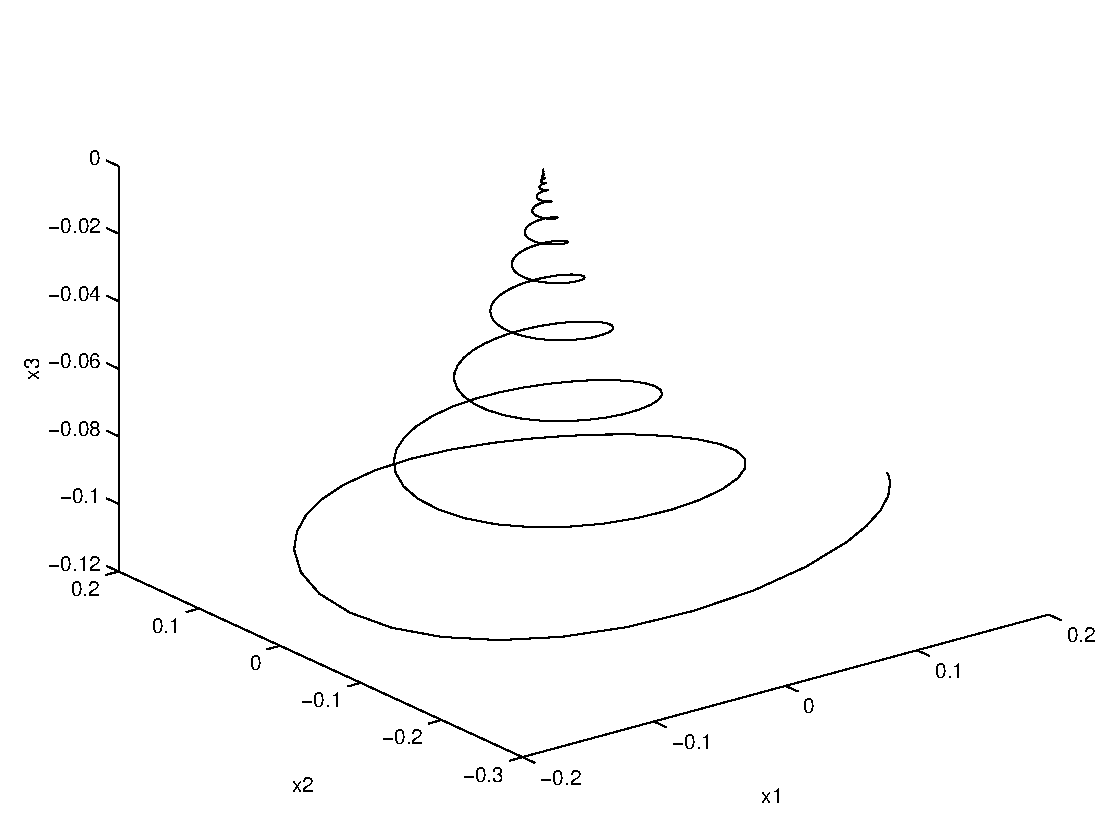
\psfig{file=../figures/fnonlin3.eps,width=5.0in}}
   \caption{Time series showing convergence to the origin for the solution of 
	the nonlinear system \protect\eqref{E:fnonlin} with initial condition 
	$X_0=(2,-1,-1)$.}
   \label{F:fnonlin3}
\end{figure*}
 
\subsection*{Periodic Solutions in Three Dimensions}

Since planar autonomous nonlinear systems produce limit cycles as solutions, 
it should come as no surprise that nonlinear three-dimensional systems can 
also have periodic solutions.  

An example of a system of differential equations having a limit cycle as a 
solution is:
\begin{matlabEquation} \label{E:3per}
\begin{array}{rcl}
\dot{x}_1 & = & -x_1 - x_2 + x_1x_3 \\
\dot{x}_2 & = &  x_1 - x_2 + x_2x_3 \\
\dot{x}_3 & = &  1 + x_3 - x_1^2 - x_2^2 - x_3^3.
\end{array}
\end{matlabEquation}
Using the m-file
\begin{verbatim}
function f = f14_4_4(t,x)
f = [-x(1) - x(2) + x(1)*x(3); 
      x(1) - x(2) + x(2)*x(3); 
        1  + x(3) - x(1)^2 - x(2)^2 - x(3)^3];
\end{verbatim}
numerically integrate \eqref{E:3per} with initial condition
$X_0=(0.5,0.4,0.3)$ by typing
\begin{verbatim}
[t,x] = ode45('f14_4_4', [0 50], [0.5,0.4,0.3]);
\end{verbatim}
Using {\tt subplot} we can plot the three time series obtaining the result in 
Figure~\ref{F:3per}.  After an initial transient, each component of the 
solution settles into a periodic motion with the same period.
\begin{figure*}[htb]
   \centerline{%
   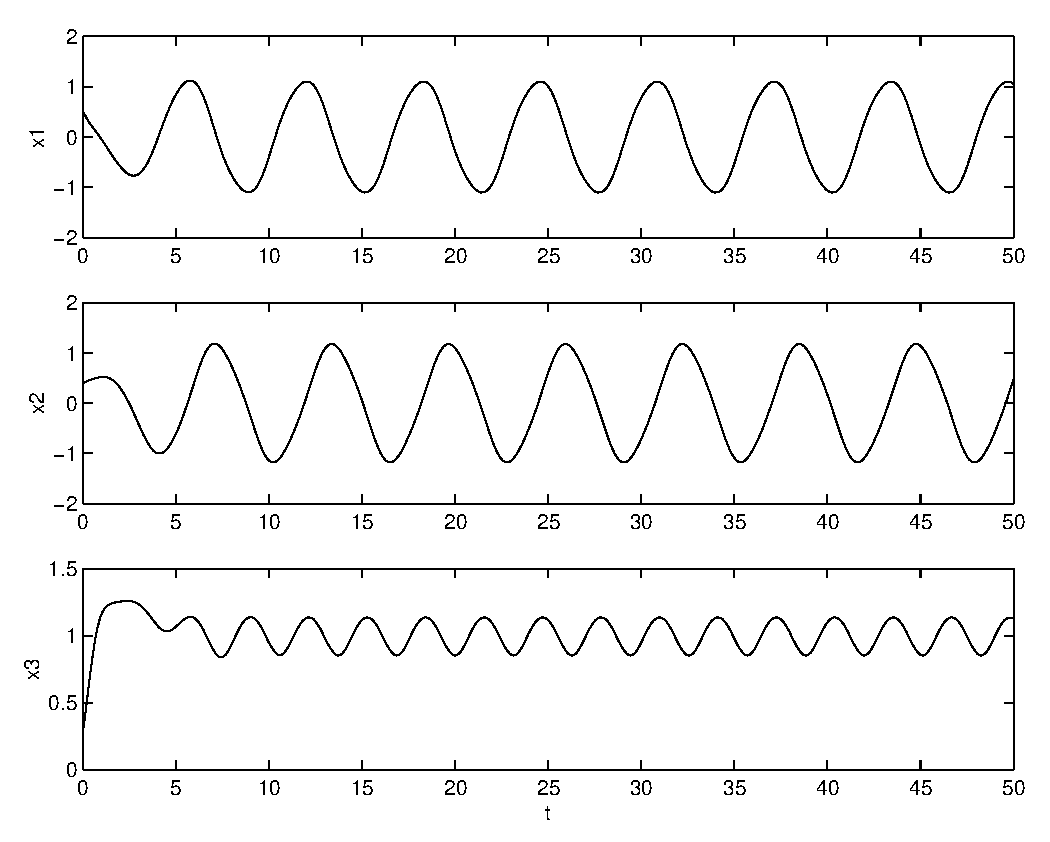
\psfig{file=../figures/f3perts.eps,width=3.0in}}
   \caption{Time series showing convergence to a limit cycle for the solution 
	of the nonlinear system \protect\eqref{E:3per} with initial condition 
	$X_0=(0.5,0.4,0.3)$.}
   \label{F:3per}
\end{figure*}

In the three-dimensional phase space $x_1,x_2,x_3$ this solution converges to a 
a simple closed curve or a deformed `circle'.  See Figure~\ref{F:3perps} 
which is reproduced using the \Matlab commands
\begin{verbatim}
plot3(x(:,1),x(:,2),x(:,3))                  
xlabel('x1')
ylabel('x2')
zlabel('x3')
\end{verbatim}

\begin{figure}[htb]
   \centerline{%
   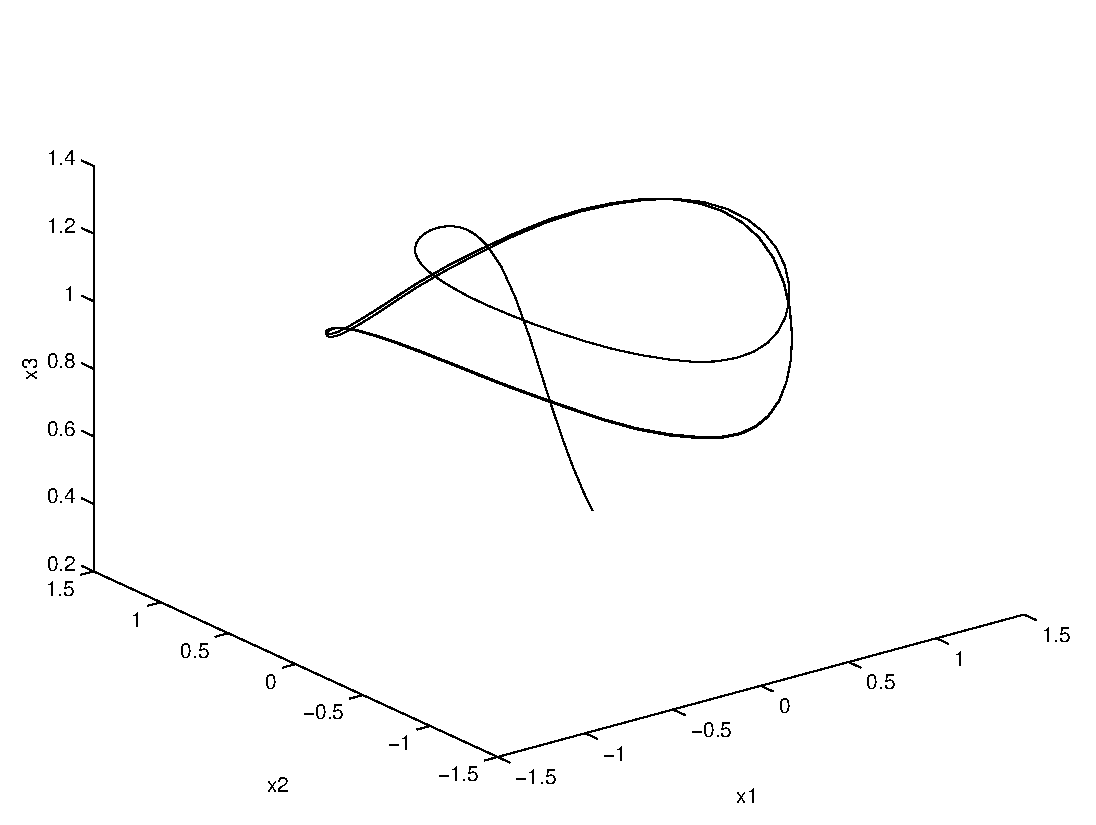
\psfig{file=../figures/f3perps.eps,width=3.0in}}
   \caption{Phase space picture showing convergence to a deformed `circle' 
	for the solution of the nonlinear system \protect\eqref{E:3per} with 
	initial condition $X_0=(0.5,0.4,0.3)$.}
   \label{F:3perps}
\end{figure}


\EXER

\includeexercises


\end{document}
